%https://github.com/milizeus/MFP-flashcards.git
%
\documentclass[a5paper,12pt,ngerman,grid=front %
%,toc % funktioniert nicht in Kombination mit print
,print
]{kartei}
\usepackage{hyperref}
\usepackage[german]{babel}
\usepackage[utf8x]{inputenc}
\usepackage{amsmath}
\usepackage{amssymb}
\usepackage{graphicx}
\usepackage[version=3]{mhchem}
\usepackage{gensymb}
\usepackage{enumitem} 
\let\oldce\ce
\renewcommand*{\ce}[1]{\begingroup\color{red}\oldce{#1}\endgroup}
%%%%%%%%%%%%%%%%%%%%%%%%%%%%%%%%%%%%%%%%%%%%%%%%%%%%%%%%%%%%%%%%%%%%%%%%%%
%%%%%%%%%%%%%%%%%%%%%%%%%%%%%%%%%%%%%%%%%%%%%%%%%%%%%%%%%%%%%%%%%%%%%%%%%%


\title{Prüfungsfragen Molekül- und Festkörperphysik}
%%%%%%%%%%%%%%%%%%%%%%%%%%%%%%%%%%%%%%%%%%%%%%%%%%%%%%%%%%%%%%%%%%%%%%%%%%


\begin{document}
\setcardpagelayout

%%%%%%%%%%%%%%%%%%%%%%%%%%%%%%%%%%%%%%%%%%%%%%%%%%%%%%%%%%%%%%%%%%%%%%%%%%
%%%%%%%%%%%%%%%%%%%%%%%%%%%%%%%%%%%%%%%%%%%%%%%%%%%%%%%%%%%%%%%%%%%%%%%%%%
\section*{Molek"ulphysik}
%%%%%%%%%%%%%%%%%%%%%%%%%%%%%%%%%%%%%%%%%%%%%%%%%%%%%%%%%%%%%%%%%%%%%%%%%%
%%%%%%%%%%%%%%%%%%%%%%%%%%%%%%%%%%%%%%%%%%%%%%%%%%%%%%%%%%%%%%%%%%%%%%%%%%



%%%%%%%%%%%%%%%%%%%%%%%%%%%%%%%%%%%%%%%%%%%%%%%%%%%%%%%%%%%%%%%%%%%%%%%%%%
	\begin{karte}{
		Skizzieren Sie die symmetrische und antisymmetrische Wellenfunktion eines 
		homonuklearen zweiatomigen Moleküls. (anti/bindende Wellenfkt.)
		}
		
		$\Psi_s=\frac{1}{\sqrt{2+2S_{AB}}}(\Phi_A+\Phi_B)$ \\
		
		$\Psi_a=\frac{1}{\sqrt{2+2S_{AB}}}(\Phi_A-\Phi_B)$ \\
		
		Mit "Überlappungsintegral": $S_{AB}=Re \int \Phi_A \Phi_B$ \\
		
		Wellenfunktion Kern A: $ \Phi_A= \frac{1}{\sqrt{a_0^3}}e^{-\frac{r_A}{a_0}}$ \\
		
		Bohrscher Atomradius: $a_0$ \\
		
		$\Psi_s$ führt zu bindenden, $\Psi_a$ zu antibindenden Zustand
		
	\end{karte}


%%%%%%%%%%%%%%%%%%%%%%%%%%%%%%%%%%%%%%%%%%%%%%%%%%%%%%%%%%%%%%%%%%%%%%%%%%
	\begin{karte}{
		Welche Überlegungen führen zur MO- und VB-Näherung?
		}
		
		Da das $\ce{H2}$ Molekül 2 Elektronen besitzt und man diese Wechselwirkung zwischen 
		den Elektronen natürlich berücksichtigen muss, führt dies zu einer nicht mehr 
		analytisch lösbaren Schrödingergleichung. 
		(Separierung der SG wie beim $\ce{He^+}$ Molekül nicht mehr möglich)
		Man muss also Näherungsmethoden finden.
		
		\begin{itemize}
			\item Molekül-Orbital Näherung 
			
			Die Überlegung ist, dass das Molekül für Atomabstand $R \rightarrow \infty$ 
			in 2 $\ce{H}$ Atome im 1s Zustand zerfällt. 
			Man kann nun also einen Ansatz mit $\ce{H}$ 1s Wellenfunktionen machen und für 
			das ganze Molekül einen Produktansatz aus 2 dieser Funktionen 
			(für Atom A und Atom B) bilden.
			
			$\Psi_{\vec{r_1},\vec{r_2}} = \Psi_s(\vec{r_1})\Psi_s(\vec{r_2})$ symmetrisch bezüglich
			Vertauschung der Elektronen, aber aus dem Pauli Prinzip
			folgt, dass die Gesamtwellenfunktion antisymmetrisch sein muss, also muss es 
			einen antisymmetrischen Spinanteil in der Gesamtwellenfunktion geben:
			
			$\Psi(\vec{r_1},\vec{r_2},\vec{s_1},\vec{s_2})=
			\Psi_s(\vec{r_1})\Psi_s(\vec{r_2})(\chi^+(1)\chi^-(2) - \chi^+(2)\chi^-(1))$
			
			Wobei man schreiben kann: 
			$\chi^+ = \alpha$, $\chi^- = \beta$ 
			(wobei $\alpha(1)$: $m_s(1) = +\frac{1}{2}$, $\beta(1): m_s(2) = -\frac{1}{2})$
			
			Wenn man nun die symmetrische Wellenfunktion 
			$\Psi= \frac{1}{\sqrt{2+2S_{AB}}}(\Phi_A+\Phi_B)$
			für die $\Psi_S(\vec{r_1} ) \Psi_S(\vec{r_2} )$ einsetzt und die Abkürzungen $\Phi_A=a$ und 
			$\Phi_B=b$ einführt bekommt man für den räumlichen Anteil:
			$  \Psi( \vec{r_1}, \vec{r_2} ) = \frac{1}{2+2S_{AB}} \left[ a(1)+b(1) \right]\left[ a(2)+b(2) \right]   $
			
		\item Valenzbindungs Näherung 
		
		Die VB-Näherung geht auch vom Molekülorbitalmodell aus. 
		Im untersten Orbital können sich dabei 2 Elektronen mit entgegengesetzten Spin aufhalten. 
		Der Ansatz ist: \\
		$\Psi_1 = c_1 \phi_A(1) \phi_B(2)$ 
		was bedeutet, dass sich Elektron 1 an Kern A und Elektron 2 an Kern B befindet, 
		aber wegen der Ununterscheidbarkeit kann auch 
		$\Psi_2 = c_1 \phi_A(2) \phi_B(1)$
		eine Lösung sein (Elektron 2 an Kern A und umgekehrt), also bildet man eine Linearkombination:
		 $\Psi_{S,A} = c[ \phi_A(1) \phi_B(2) \pm \phi_A(2) \phi_B(1) ] $ 
			 
			
		\end{itemize}
		
	\end{karte}
		
		
%%%%%%%%%%%%%%%%%%%%%%%%%%%%%%%%%%%%%%%%%%%%%%%%%%%%%%%%%%%%%%%%%%%%%%%%%%
	\begin{karte}{
		Vergleiche Molekülorbitale und Valenzbindungsmodelle (Heitler London Näherung).
		}
		
		\begin{itemize}
			\item Molekül-Orbital Näherung \\
			
			Die Überlegung ist, dass das Molekül für Atomabstand $R \rightarrow \infty$ in 2 
			$\ce{H}$ Atome im 1s Zustand zerfällt. 
			Man muss nun also einen Ansatz mit $\ce{H}$ 1s Wellenfunktionen machen und für 
			das ganze Molekül einen Produktansatz aus 2 dieser Funktionen 
			(für Atom A und Atom B) bilden. \\
			Mit Beachtung des Pauli-Prinzips folgt dann:
			$\Psi_{\overrightarrow{r_1},\overrightarrow{r_2}} = \frac{1}{2+2S_{AB}}[a(1)+b(1)][a(2)+b(2)]$
			
			\item Valenzbindungs Näherung \\
			 
			 Bei der VB geht man von Molekükorbitalen aus, also setzt man direkt eine Wellenfunktion für 2 Elektronen an. Durch die Forderung, dass die Wellenfunktion entweder symmetrisch oder antisymmetrisch ist, folgt der Ansatz einer Linearkombination beider möglichen Lösungen.
			 $ \Psi_1 = c_1\phi_A(1)\phi_B(2) $ und $ \Psi_2 = c_1\phi_A(2)\phi_B(1) $ zu
			 $$  \Psi_{S,A} = c \left[   \phi_A(1) \phi_B(2) \pm   \phi_A(2) \phi_B(1)   \right]  $$
			 
			 Wenn man die Klammern in der MO Gleichung ausmultipliziert, sieht man, dass im VB Ansatz die Terme, die beschreiben, dass sich beide Elektronen entweder an Kern A oder Kern B befinden, fehlen.
			 Jetzt ist dieser Zusand zwar unwahrscheinlicher als die anderen Zustände, wird aber in der MO mit gleicher Stärke berücksichtigt. Die VB berücksichtigt dafür diese Terme gar nicht.
			 Ansonsten sind die Näherungen gleich.
			
		\end{itemize}
		
	\end{karte}
	
	
%%%%%%%%%%%%%%%%%%%%%%%%%%%%%%%%%%%%%%%%%%%%%%%%%%%%%%%%%%%%%%%%%%%%%%%%%%
	\begin{karte}{
		Erläutere die Verbesserung des MO-Ansatzes.
		}

		Der ionische Zustand der Wellenfunktion $\left(  (a(1)a(2) + b(1)b(2) \right) $
		, der in VB gar nicht und in MO mit gleicher Stärke wie die anderen Terme vorkommt, wird über eienen Parameter $ 0 < \lambda < 1 $ in die Wellenfunktion eingebaut.
		$$ \Psi = c[ a(1)b(2) + a(2)b(1) + \lambda[ a(1)a(2) + b(1)b(2) ] ] $$
		Wenn man nun $\lambda$ so variiert, dass man für jeden Kernabstand $R$ eine minimale Gesamtenergie $E(R)$ erhält, bekommt man eine Bindungsenergie $ \Delta E(R_e) = -4.02eV $, was schon sehr viel besser dem realen Wert enstspricht.
		Man kann nun aber noch beachten, dass sich die Atomorbitale bei der Annäherung der $\ce[H]$ Atome verformen. Deshalb setzt man statt 
		$$ \Psi_S = \frac{1}{\sqrt{2+2S_{AB}}} (\phi_A + \phi_B) $$
		eine Linearkombination aus $N$ atomaren Orbitalen ein:
		$$ \Psi = \sum_{i=1}^{N} c_i\phi_i $$
		
		Als Molekülorbital kann man dann entweder einen MO Ansatz $$\Psi = \Psi_1 \Psi_2$$
		
		oder einen VB Ansatz wählen $$ \Psi = \sum_{i,k} c_i\phi_i(1)c_k\phi_k(2) $$
		
		In beiden Fällen versucht man dann durch variieren der Koeffizienten die Gesamtenergie für jeden Kernabstand zu minimieren. Mit diesem Ansatz kommt man experimentellen Wert dann bereits sehr nahe.
		
	\end{karte}
	
	
%%%%%%%%%%%%%%%%%%%%%%%%%%%%%%%%%%%%%%%%%%%%%%%%%%%%%%%%%%%%%%%%%%%%%%%%%%
	\begin{karte}{
		Warum ist $\ce{He2+}$ stabil aber $\ce{He2}$ nicht?
		}
		
		Beim $\ce{He2}$ werden die $2e$ im $1s \sigma_g$ Orbital (bindend) praktisch komplett durch die zwei $e^-$ im antibindenden $1s\sigma_u$ Orbital kompensiert. 
		Es gibt aber $\ce{He2^*}$ bei dem ein $e^-$ im $1s\sigma_u$ angeregt wird. 
		Dieses ist wieder stabil. \\
		
		Beim $\ce{He2^+}$ fehlt ein $e^-$ und es kann deshalb zu keiner totalen Kompensation der Bindung kommen und damit ist es auch stabil.
				
	\end{karte}


%%%%%%%%%%%%%%%%%%%%%%%%%%%%%%%%%%%%%%%%%%%%%%%%%%%%%%%%%%%%%%%%%%%%%%%%%%
	\begin{karte}{
		Warum ist das $\ce{H2}$ Molekül, nicht aber das $\ce{He2}$ Molekül stabil?
		}
		
		Das $\ce{He}$ Molekül besitzt $2e$ im $1s\sigma_g$ Orbit. \\
		Beim $ \ce{He2} $ hat man aber $2e$ im $1s \sigma_g$ und $2e$ im $1s\sigma_u$. \\
		Diese kompensieren sich und das Molekül ist, im Gegensatz zu $\ce{H2}$, nicht stabil.
		
	\end{karte}


%%%%%%%%%%%%%%%%%%%%%%%%%%%%%%%%%%%%%%%%%%%%%%%%%%%%%%%%%%%%%%%%%%%%%%%%%%
	\begin{karte}{
		Diskutieren Sie die Bindung im $\ce{Na2}$ Molekül.
		}
		

		\begin{figure}[htbp]
			\centering
			\includegraphics[width=0.5\linewidth]{./images/07_Na2}
			\caption[Na2]{$Na_2: [K][K]  (2s \sigma_g)^2 (2s \sigma_u)^2  (2 \sigma \pi_u)^6 (2 \sigma \pi_g)^6 (3s \sigma_g)^2  $}
		\end{figure}

		
	\end{karte}


%%%%%%%%%%%%%%%%%%%%%%%%%%%%%%%%%%%%%%%%%%%%%%%%%%%%%%%%%%%%%%%%%%%%%%%%%%
	\begin{karte}{
		Diskutieren Sie die Bindung im $\ce{Li2}$ und $\ce{CH4}$ Molekül.
		}
		
		\begin{figure}[htbp]
			\centering
			\includegraphics[width=0.3\linewidth]{./images/08_Li2}
			\caption[Li2]{$Li_2: [K][K]  (1s \sigma_g)^2 (1s \sigma_u)^2  (2s \sigma_g )^2   $}
		\end{figure}
		
	\end{karte}


%%%%%%%%%%%%%%%%%%%%%%%%%%%%%%%%%%%%%%%%%%%%%%%%%%%%%%%%%%%%%%%%%%%%%%%%%%
	\begin{karte}{
		Diskutiere die chemische Bindung im $\ce{B2}$ Modell.
		}
		
		\begin{figure}[htbp]
			\centering
			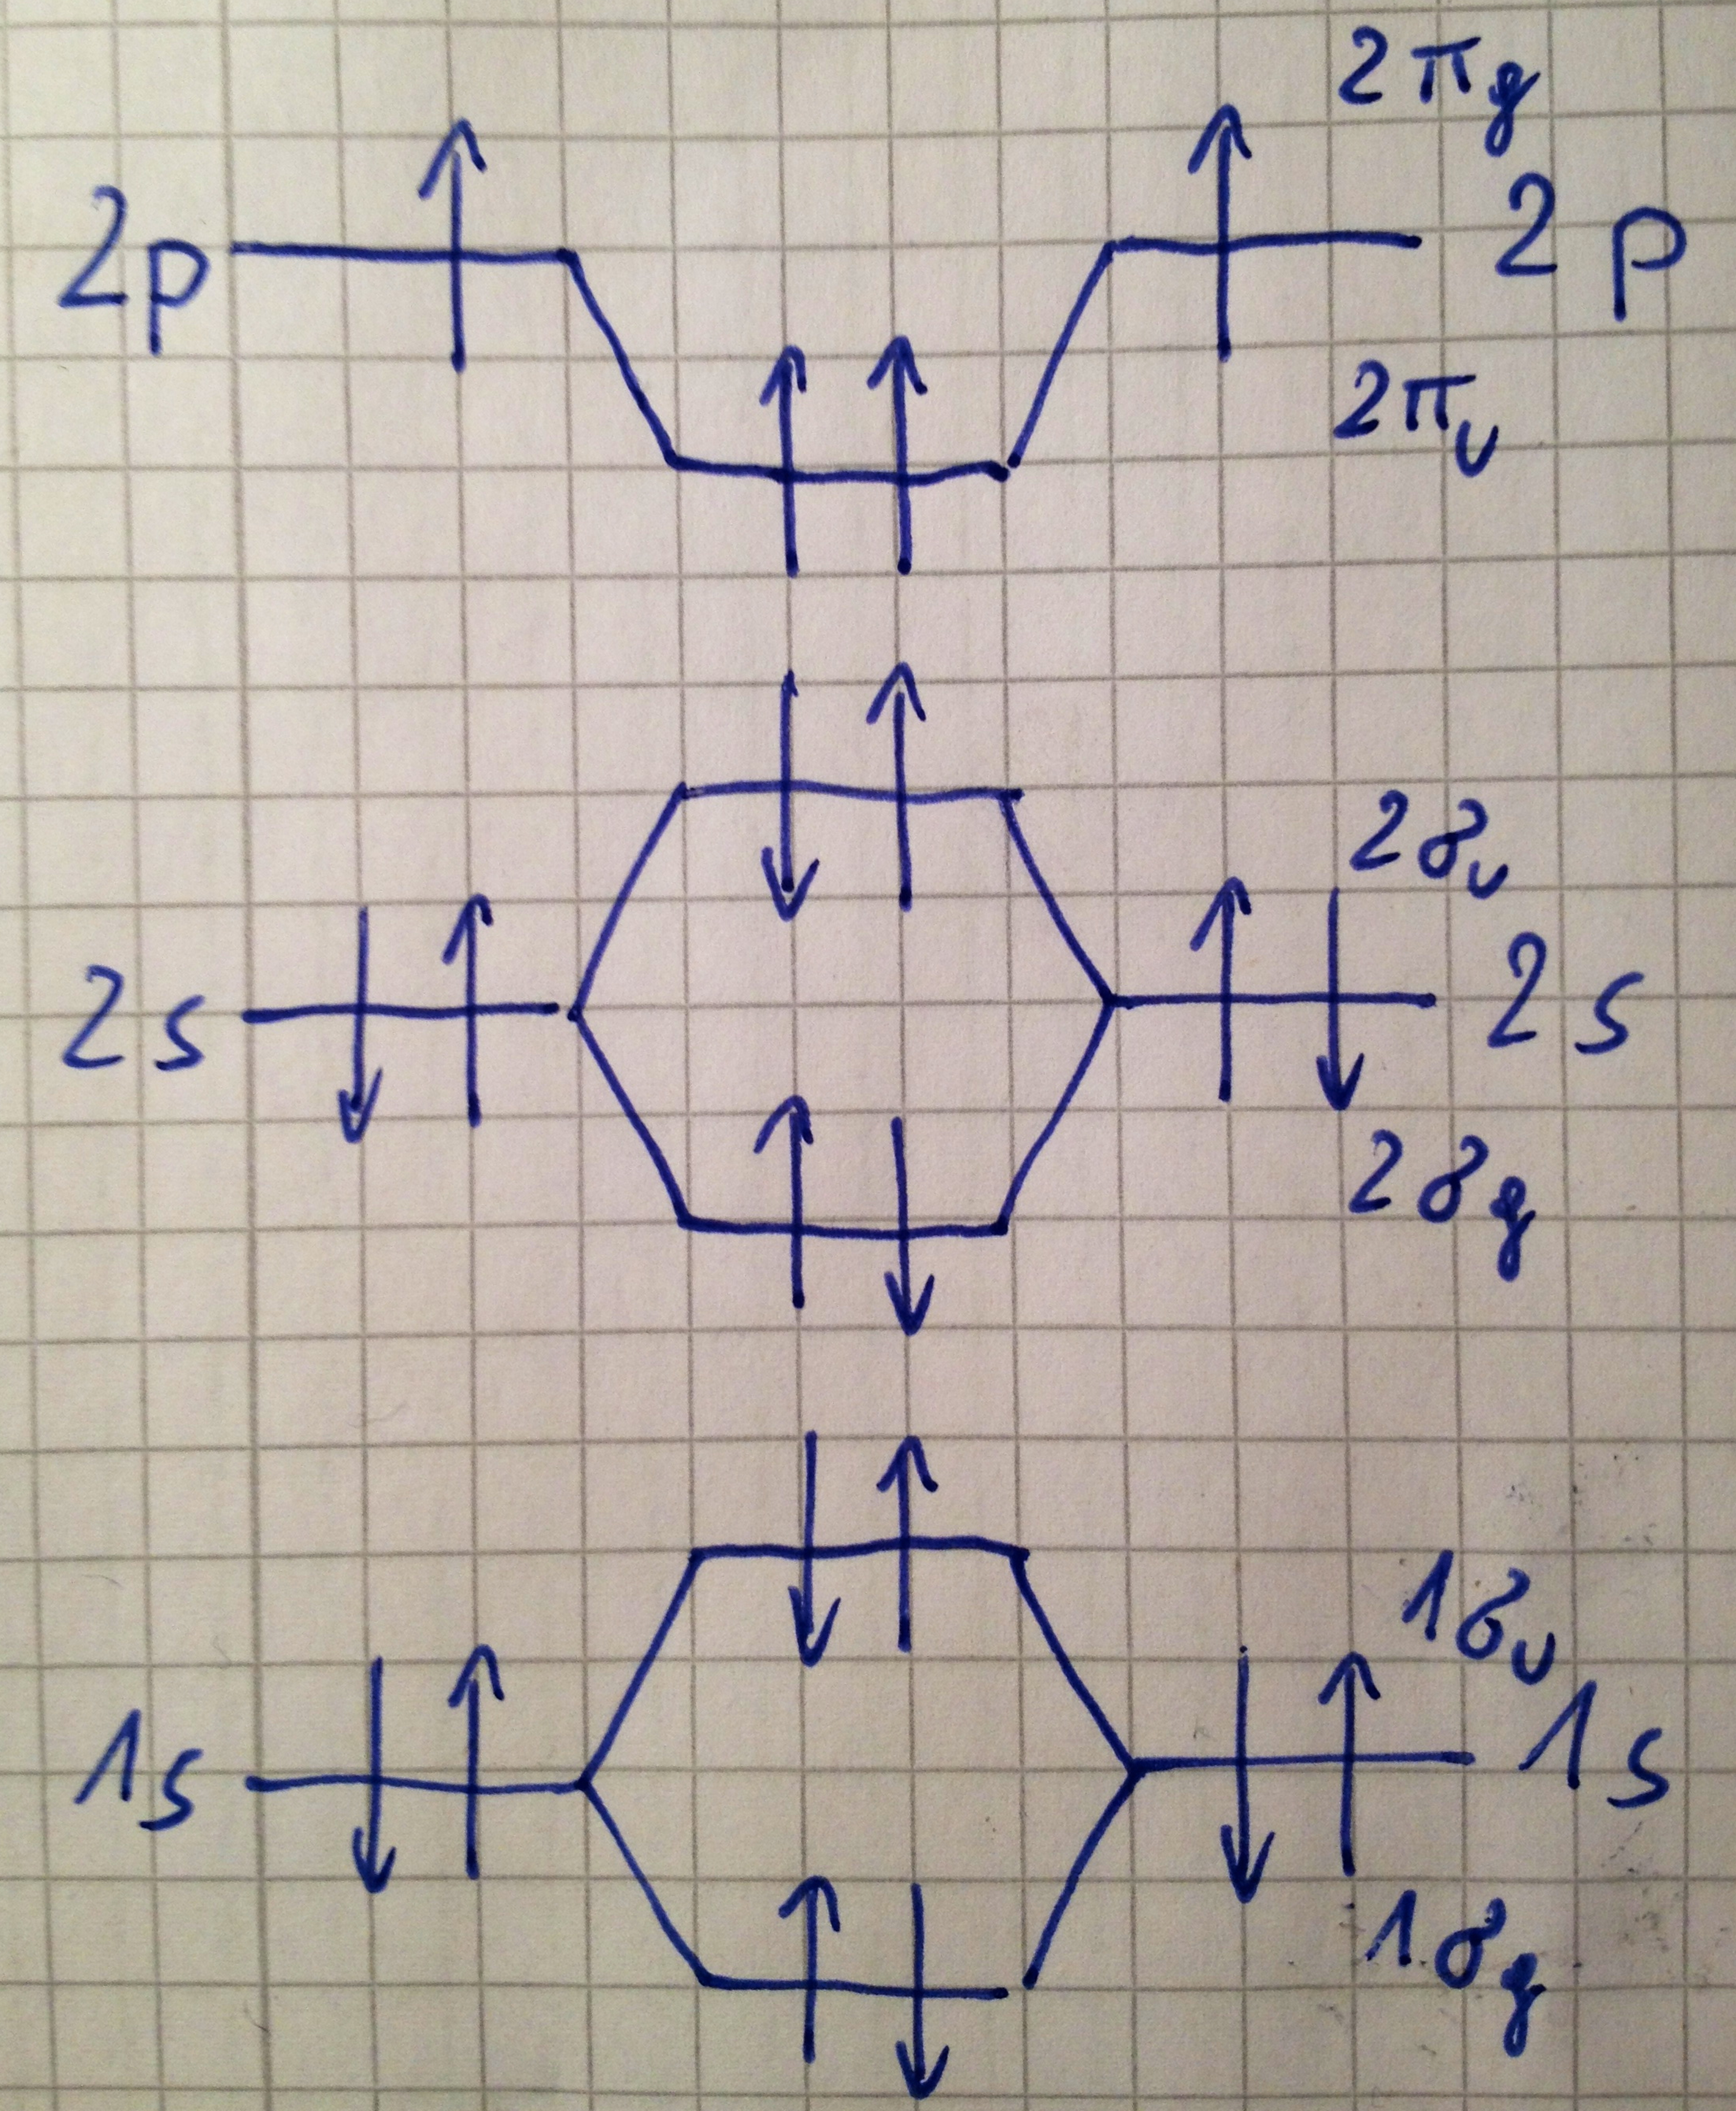
\includegraphics[width=0.3\linewidth]{./images/09_B2}
			\caption[Li2]{$B_2: [K][K]  (2s \sigma_g)^2 (2s \sigma_u)^2  (2p \pi_u )^2   $}
		\end{figure}
		
	\end{karte}


%%%%%%%%%%%%%%%%%%%%%%%%%%%%%%%%%%%%%%%%%%%%%%%%%%%%%%%%%%%%%%%%%%%%%%%%%%
	\begin{karte}{
		Molekülbindungsarten? (kovalente, ionische, Valenzbindung)
		}
		
		\begin{itemize}
			\item Kovalente Bindung \\
				Erfolgt durch den Austausch gemeinsamer Elektronen zwischen den 2 Atomen und führt zu einer Umordnung der Elektronendichteverteilung. \\
				Coulomb Wechselwirkung, \\
				Austausch Wechselwirkung, \\
				nur bei Kernabständen $ R<r_1+r_2 $
				
			\item Ionenbindung \\
				Bindung zwischen negativen und positiven Ionen. Sie tritt auf, wenn es durch Elektronenaustausch zu einer erhöhten Elektronendichte in Atom A und einer geringeren an Atom B kommt.\\
				Fällt mit $ \dfrac{1}{R} $ ab, also langreichweitig.
			\item Wasserstoff-Brücken Bindung \\
				Anziehung zwischen 2 Atomen durch ein $\ce{H+}$ Ion. \\
				Das Proton polarisiert die beiden Atome und dies führt zu einer anziehenden Kraft.
			\item Van der Waals Bindung \\
				Zwischen 2 neutralen polarisierbaren Atomen.\\
				Es bildet sich ein Dipol und dies führt zu einer schwachen und kurzreichweitigen Bindung. \\
				$\dfrac{1}{R^6}$
		\end{itemize}
		
	\end{karte}


%%%%%%%%%%%%%%%%%%%%%%%%%%%%%%%%%%%%%%%%%%%%%%%%%%%%%%%%%%%%%%%%%%%%%%%%%%
	\begin{karte}{
		Beschreiben sie die Elemente der Born-Openheimer Näherung.
		}
		
		Näherung zur Berücksichtigung nicht starrer Moleküle. \\
		
		Wegen der viel größeren Masse der Kerne läuft deren Bewegung viel langsamer als die der Elektronen ab. Die Elektronen könne sich praktisch instantan auf den Kernanstand einstellen.\\
		
		Weiters hängt die Elektronenenergie zwar von $R$ ab, wird aber durch die Bewegung des Kerns kaum beeinflusst. \\
		
		Die Wellenfunktion lässt sich dadurch als Produkt aus Kern- und Elektronenwellenfunktion schreiben. \\
		
		Beim Einsetzen in die SG erhällt man dann die Gleichung für die elektronische Wellenfunktion des starren Moleküls und eine Gleichung für die Bewegung des Kerns in einem Potential. \\
		
		Diese Näherung ist nur für schwere Moleküle im Grundzustand geeignet.
		
		
	\end{karte}


%%%%%%%%%%%%%%%%%%%%%%%%%%%%%%%%%%%%%%%%%%%%%%%%%%%%%%%%%%%%%%%%%%%%%%%%%%
	\begin{karte}{
		Beschreibe die Rotation zweiatomiger Moleküle.
		}
		
		Quasiklassischer Ansatz: Rotation um Achse durch den Schwerpunkt. \\
		Bei Massen $M_1$, $M_2$ und Winkelgeschwindigkeit $\omega$ ist die Rotationsenergie 
		$$E_{rot} = \frac{1}{2} I \omega^2 = \frac{\vec{J}^2}{2 I}$$
		
		mit \\
		$ |\vec{J}|=I \omega  $ \\
		$ I = M_1 R_1^2 + M_2 R_2^2 = M R^2 $
		
		wobei \\
		$ M = \frac{M_1 M_2}{M_1 + M_2} $ „reduzierte Masse“ \\
		und \\
		$ |\vec{J}^2| = J(J+1){\hslash}^2 $ aus QM, \\
		erhällt man beim Gleichgewichtsabstand $ R = R_e $ \\
		
		$$ E_{rot} = \frac{J(J+1)\hslash^2}{2 M R_e^2}  $$
		
		Es kann damit nur diskrete Abstände der Rotationsenergieniveaus geben:
		
		$$       \Delta E_{rot} = E_{rot} (J+1) - E_{rot} (J) = \frac{( J+1 ) \hslash^2 }{ I }       $$
		
	\end{karte}


%%%%%%%%%%%%%%%%%%%%%%%%%%%%%%%%%%%%%%%%%%%%%%%%%%%%%%%%%%%%%%%%%%%%%%%%%%
	\begin{karte}{
		Vorteile Morse-Potential gegenüber harmonischem Potential.
		}
		
		\begin{itemize}
			\item harmonisches Potential \\
				Das harmonische Potential beschreibt mit seiner Parabelform zwar gut das Potential eines rotierenden Moleküls in der Nähe des Gleichgewichtabstandes $R=R_e$, aber für höhere Energien ist die Näherung nicht besinders gut, da das harmonische Potential für $R \rightarrow \infty$ gegen $ E \rightarrow \infty $ strebt, obwohl es eigentlich gegen die Dissoziationsenergie $E_D$ konvergieren sollte.
				
			\item Morse-Potential \\
				Das Morse-Potential ist besser, da es näher am wirklichen Potential liegt und darüber hinaus, noch immer analytisch lösbar ist. Es konvergiert auch wirklich gegen $E_D$ und besitzt ein Minimum bei $R=R_e$
				$$ E_{pot}(R) = E_D[ 1-e^{ -a( R-R_e ) } ]^2 $$
				
		\end{itemize}
		
	\end{karte}


%%%%%%%%%%%%%%%%%%%%%%%%%%%%%%%%%%%%%%%%%%%%%%%%%%%%%%%%%%%%%%%%%%%%%%%%%%
	\begin{karte}{
		Wovon hängt die Intensität einer Spektrallinie ab?
		}
		
		Die Intensität hängt von der Übergangswahrscheinlichkeit ab.
		
		Je höher die Wahrscheinlichkeit, desto intensiver die Linien.
		
		Intensität $\propto$ Übergangswahrscheinlichkeit $\propto$ $|M_{ij}|^2$ „Übergangsmatrixelement“
		
	\end{karte}


%%%%%%%%%%%%%%%%%%%%%%%%%%%%%%%%%%%%%%%%%%%%%%%%%%%%%%%%%%%%%%%%%%%%%%%%%%
	\begin{karte}{
		Diskutiere das Schwingungs-Rotations-Spektrum bei zweiatomigen Molekülen.
		}
		
		Übergänge zwischen Schwingungs-Rotations Niveaus $ (v_i, \vec{J}_i ) $ und $ (v_j, \vec{J}_j ) $ innerhalb des selben elektronischen Zustandes bilden für $ v_i \neq v_j $ das Schwingungs-Rotations Spektrum, das im infraroten Spektralbereich liegt (bei $ v_i = v_j $ nur Rotationsspektrum im Mikrowellenbereich)
		
	\end{karte}


%%%%%%%%%%%%%%%%%%%%%%%%%%%%%%%%%%%%%%%%%%%%%%%%%%%%%%%%%%%%%%%%%%%%%%%%%%
	\begin{karte}{
		Wovon hängt die Intensität bei einem elektronischen Übergang ab?
		}
		
		Da die Übergangswahrscheinlichkeit $ \propto |\vec{M_{ik}}|^2 $ ist, ist die Intensität $ I \propto |\vec{M_{ik}^{el}}|^2 FC(v_i, v_k) HL(J_i, J_k)  $. 
		\\
		Wobei die einzelnen Faktoren folgendes sind: \\
		\begin{itemize}
			\item Der elektronische Anteil $ |\vec{M_{ik}} |^2 $ der die Wahrscheinlichkeit für einen Elektronenübergang von $ | i > $ nach $ |k> $ angibt. Dieser Teil hängt vom Überlapp der elektronischen Wellenfunktion ab.
			\item Der Frank-Condon-Faktor
			$$  FC(v_i,v_j) = \left|    \int  \psi_{vib}(v_i)    \psi_{vib}(v_k)  dR  \right| ^2     $$
			der gleich dem Absolutquadrat des Überlapps der Schwingungswellenfunktionen im oberen und unteren Zustand ist.
			\item Der Hönl-London-Faktor
			$$   HL(  J_i, J_k  )  =  \left|    \int Y_{J_{i}}^{ M_i }    Y_{J_{k}}^{ M_k } \vec{p} \sin(\theta) d\theta d\phi    \right|^2    $$
			der gleich dem Absolutquatrat des Überlapps der Rotationswellenfunktionen im oberen und unteren Zustand ist.
		\end{itemize}
		Bem.: Nur wenn keiner der Faktoren 0 ist kann ein elektronischer Überlapp stattfinden.
	\end{karte}
	
	
%%%%%%%%%%%%%%%%%%%%%%%%%%%%%%%%%%%%%%%%%%%%%%%%%%%%%%%%%%%%%%%%%%%%%%%%%%


	\begin{karte}{
		Franck-Condon-Prinzip und Intensität des Schwingungsüberganges.
		}
		
		Die Absorbtion/Emission eines Photons und damit ein Übergang zwischen Zuständen passiert in einer Zeit, die klein ist gegenüber der Schwingungsdauer der Kerne. Dadurch erfolgt der Übergang im Energie/Kernabstand Diagramm senkrecht. Nun ist die Wahrscheinlichkeit für einen Übergang abhängig vom Fanck-Condon-Faktor:
		$$  FC(v_i, v_j) = \left|   \int  \Psi_{ vib } (v_i)  \Psi_{ vib } (v_k)  dR    \right|^2   $$
		
		Wenn jetzt die Potentialkurven im oberen und unteren Zustand ähnlich sind und die Minima bei gleichen Kernabstand liegen, sind Übergänge $ \Delta v = v'- v''= 0 $ am wahrscheinlichsten. Sind aber die Potentialkurven zu einander verschoben sind Übergänge $ \Delta v \neq 0 $ am wahrscheinlichsten und haben damit die größte Intensität. Je größer die Verschiebung zwischen den Potentialkurven desto größer werden die wahrscheinlichsten $\Delta v$.
		
		\begin{figure}[htbp]
			\centering
			\includegraphics[width=0.4\linewidth]{./images/17_FCP}
			\caption{Franck-Condon-Prinzip}
		\end{figure}
		
		
	\end{karte}


%%%%%%%%%%%%%%%%%%%%%%%%%%%%%%%%%%%%%%%%%%%%%%%%%%%%%%%%%%%%%%%%%%%%%%%%%%
	\begin{karte}{
		Diskutiere den Aufbau eines $\ce{H2O}$ Molekül.
		}
		
		Beim Wassermolekül stehen folgende Orbitale für Bindungen zur Verfügung: \\
		$  2 \times \ce{H} = 1s  $ \\
		$  1 \times \ce{O} = [K] 2s^2 2p_x^1 2p_y^1 2p_z^2  $ \\
		Wenn man nun den Ansatz mit Spin macht, dass bei 2 der $ \ce{O} $-Orbitale (z.B.: $p_x$, $p_y$) sich ein \ce{H} Atom bindet, kommt man auf einen Bindungswinkel von $90\degree$.
		Experimente zeigen aber einen Bindungswinkel von $105\degree$. Also kann dieses einfache Modell nicht ganz korrekt sein. \\
		
		Die Erklärung ist, dass sich die Elektronenhüllen der Atome bei der Bindung verformen und es dadurch zu einer veränderten Ladungsverteilung und einem größeren Überlapp der Wellenfunktionen kommt. Es bilden sich sogenante Hypbridorbitale für die die Bindungsenergie zwischen $\ce{H}$ und $\ce{O}$ maximal und die Gesamtenergie minimal wird. Dieser Ansatz erklärt auch den Bindugswinkel von $105\degree$.
		
		
	\end{karte}


%%%%%%%%%%%%%%%%%%%%%%%%%%%%%%%%%%%%%%%%%%%%%%%%%%%%%%%%%%%%%%%%%%%%%%%%%%
	\begin{karte}{
		Diskutiere den Aufbau eines $\ce{CH4}$ Moleküls im Rahmen der Molekularorbitalnäherung.
		}
		
		\begin{figure}[htdp]%
			\centering
			\begin{minipage}{0.3\textwidth}%
				\centering%
				\includegraphics[width=\textwidth]%
				{./images/18_CH4}
				\caption{$\ce{CH4}$}
			\end{minipage}%
			\hspace{0.5cm}
			%
			\begin{minipage}{0.3\textwidth}%
				\centering
				\includegraphics[width=\textwidth]%
				{./images/18_CH4_2}
				\caption{$\ce{CH4}$}
			\end{minipage}%
			%
		\end{figure}
		
	\end{karte}


%%%%%%%%%%%%%%%%%%%%%%%%%%%%%%%%%%%%%%%%%%%%%%%%%%%%%%%%%%%%%%%%%%%%%%%%%%
	\begin{karte}{
		Beschreibe das $\ce{NH3}$ Molekül.
		}
		
		Das $\ce{N}$ Atom hat 3 ungepaarte $2p$ Elektronen in den 3 $p$ Orbitalen $( p_x, p_y, p_z )$. 
		Also sollte sich eingentlich mit den $1s$ Orbitalen der $ \ce{H} $ Atome ein Bindungswinkel von $90\degree$ ergeben.
		Wie auch bei $ \ce{H2O} $ wird aber der Winkel durch Hybritisierung vergrößert. $ (107.8\degree) $.
		Die Struktur des Moleküls entspricht einer dreiseitigen Pyramide. \\
		
		Die potentielle Energie als Funktion der Höhe $h$ hat ein Maximum bei $ h=0 $ und jeweils ein Minimum bei $ h = \pm h_0 $. 
		Damit kann sich das $\ce{N}$ Atom entweder oberhalb oder unterhalb der Ebene befinden. Da diese Konfigurationen aber äquivalent sind, sind sie ununterscheidbar.
		
		\begin{figure}[htbp]
			\centering
			\includegraphics[width=0.45\linewidth]{./images/20_NH3}
			\caption{$ \ce{NH3} $}
		\end{figure}
		
	\end{karte}


%%%%%%%%%%%%%%%%%%%%%%%%%%%%%%%%%%%%%%%%%%%%%%%%%%%%%%%%%%%%%%%%%%%%%%%%%%
	\begin{karte}{
		Erklären Sie die Hybridisierung anhand des Benzol-Molekül.
		}
		
		Aus Experimenten kennt man den Aufbau des Benzol $ \ce{C6H6} $ Moleküls. Es bildet ein planares Molekül wobei die $\ce{C}$ Atome ein Sechseck bilden, an je ein $\ce{H}$ Atom gebunden ist.
		
		Der Winkel zwischen den $\ce{C}$ Atomen ist $120\degree$, dies weißt auf eine $sp^2$ Hybritisierung der Elektronen der $\ce{C}$ Atome hin.
		
		Man hat dabei also $sp^2$ Bindungen zwischen $ \ce{C-C} $ und $ \ce{C-H} $ aber auch delokalisierte $\pi$-Orbitale, die sich über den ganzen $\ce{C}$ Ring erstrecken.
		
		\begin{figure}[htdp]%
			\centering
			\begin{minipage}{0.35\textwidth}%
				\centering%
				\includegraphics[width=\textwidth]%
				{./images/21_C6H6}
				\caption{$\ce{CH4}$}
			\end{minipage}%
			\hspace{0.5cm}
			%
			\begin{minipage}{0.35\textwidth}%
				\centering
				\includegraphics[width=\textwidth]%
				{./images/21_C6H6_hyb}
				\caption{$\ce{CH4}$ Hybritisierung}
			\end{minipage}%
			%
		\end{figure}
		
	\end{karte}


%%%%%%%%%%%%%%%%%%%%%%%%%%%%%%%%%%%%%%%%%%%%%%%%%%%%%%%%%%%%%%%%%%%%%%%%%%
	\begin{karte}{
		Was sind die Normalkoordinaten bei der Beschreibung der Schwingungen mehratomiger Moleküle?
		}
		
		Koordinaten $Q$, die Schwingungen in einem mehratomigen Molekül beschreiben ohne den Schwerpunkt zu verändern.
		
		Sie beschreiben den Abstand vom Gleichgewichtsabstand.
		
		Definition über potentielle Energie:
		
		$$  U = \frac{1}{2} \sum_i \lambda_i Q_i  $$
		
	\end{karte}




%%%%%%%%%%%%%%%%%%%%%%%%%%%%%%%%%%%%%%%%%%%%%%%%%%%%%%%%%%%%%%%%%%%%%%%%%%
%%%%%%%%%%%%%%%%%%%%%%%%%%%%%%%%%%%%%%%%%%%%%%%%%%%%%%%%%%%%%%%%%%%%%%%%%%
\section*{Festkörperphysik}
%%%%%%%%%%%%%%%%%%%%%%%%%%%%%%%%%%%%%%%%%%%%%%%%%%%%%%%%%%%%%%%%%%%%%%%%%%
%%%%%%%%%%%%%%%%%%%%%%%%%%%%%%%%%%%%%%%%%%%%%%%%%%%%%%%%%%%%%%%%%%%%%%%%%%



%%%%%%%%%%%%%%%%%%%%%%%%%%%%%%%%%%%%%%%%%%%%%%%%%%%%%%%%%%%%%%%%%%%%%%%%%%
	\begin{karte}{
		Festkörperbindungsarten? (Diskutiere die metallische Bindung.)
		}
		
		Bei der metallischen Bindung sind die Wellenfunktionen im Vergleich zum Atomabstand sehr ausgedehnt $( \Psi > R )$. Es bilden sich Valenzbänder die nicht vollständig besetzt sind und es bilden sich quasi frei bewegliche Elektronen im Gitter. Diese führen zur guten Leitfähigkeit von Metallen. Dieses partiell gefüllte Valenzbandkann auf verschiedene Arten entstehen:
		\begin{itemize}
			\item kovalente Bindung
			\item metallische Bindung
				\item Alkalimetalle:
					s-Band nur $1/2$ gefüllt. z.B.: $\ce{Li}$, $\ce{Na}$, $\ce{K}$, $\ce{Rb}$, $\dots$
				\item Erdalkalimetalle:
					s-Band gefüllt. Es bildet sich wegen der Überlappung der s-Bänder mit den p-Bändern praktisch nur ein sp-Band
				\item Übergangsmetalle:
					sp Zustände bilden wieder ein gemeinsames Band (breit $\Rightarrow$ Leitfähigkeit) \\
					weiters noch d-Band (schmal, kovalente Anteile an der Bindung)
			\item Ionenbindung
			\item Wasserstoffbrückenbindung
			\item Van der Waals Bindung
		\end{itemize}
			
	\end{karte}


%%%%%%%%%%%%%%%%%%%%%%%%%%%%%%%%%%%%%%%%%%%%%%%%%%%%%%%%%%%%%%%%%%%%%%%%%%
	\begin{karte}{
		Graphit versus Diamant: Wodurch unterscheidet sich die chemische Bindung in diesen
		beiden Festkörpern?
		}
		
		Beide bestehen aus reinem Kohlenstoff(sofern man mögliche Verunreinigungen vernachlässigt). 
		
		\begin{itemize}
			\item Die Struktur des Diamanten besteht aus 2 sich durchdringende kubisch flächenzentrierte (fcc) Gitter, wobei jedes $\ce{C}$ Atom mit 4 Nachbarn kovalent gebunden ist. Es ist damit das härteste Mineral.
			
			\item Beim Graphit besteht die Kristallstruktur aus hexagonalen Gittern (hexagonal dichteste Kugelpackung, hcp). Die Atome sind in den Ebenen kovalent gebunden, wobei sich eine $sp^2$ Hybritisierung ergibt. Diese Bindung ist, im Gegensatz zur Bindung zwischen den Ebenen sehr stark. Damit ergibt sich eine große Richtungsabhängigkeit der Härte des Graphits.
			
		\end{itemize}
		
	\end{karte}


%%%%%%%%%%%%%%%%%%%%%%%%%%%%%%%%%%%%%%%%%%%%%%%%%%%%%%%%%%%%%%%%%%%%%%%%%%
	\begin{karte}{
		Unterschied zwischen fcc und hcp?
		}
		
		Fcc und hcp haben beide einen Verpackungsfaktor von 0,74, bestehen aus dicht gepackten Ebenen von Atomen und haben eine Koordinationszahl von 12. Der Unterschied zwischen der fcc und hcp ist die Stapelfolge. 
		
		Ausgehend von einer Kugel in einer dichtest gepackten Schicht A (diese eine Kugel berührt jeweils sechs andere Kugeln in der Ebene), kann diese Schicht entweder die Grundfläche einer hcp-Struktur sein, oder die diagonale Ebene der fcc-Struktur. In folgender Grafik ist veranschaulicht, warum dass fcc- und hcp-Gitter aufgrund ihrer Stapelfolgen (A, B und C sind jeweils dichtest gepackte Schichten) herausstechen
		
		\begin{figure}[htdp]%
			\centering
			\begin{minipage}{0.35\textwidth}%
				\centering%
				\includegraphics[width=\textwidth]%
				{./images/25_fcc-hcp}
				\caption{fcc vs. hcp}
			\end{minipage}%
			\hspace{0.5cm}
			%
			\begin{minipage}{0.45\textwidth}%
				\centering
				\includegraphics[width=\textwidth]%
				{./images/25_bcc-fcc-hcp}
				\caption{bcc, fcc, hcp}
			\end{minipage}%
			%
		\end{figure}
		
	\end{karte}


%%%%%%%%%%%%%%%%%%%%%%%%%%%%%%%%%%%%%%%%%%%%%%%%%%%%%%%%%%%%%%%%%%%%%%%%%%
	\begin{karte}{
		Vergleiche bcc- und fcc-Gitter.
		}
		
		\begin{itemize}
			\item bcc: body centered cubic \\
				Anordnung in einem Kubus mit Atomen in den Ecken und einem Atom im Zentrum des Würfels.
				Koordinatenzahl ist 8. \\
				Grundsätzlich wäre eine Bindung in dieser Struktur weniger wahrscheinlich, kommt aber dennoch (z.B.: alle Alkaline Metalle) oft vor.\\
				Grund: die 6 übernächsten Nachbarn sind nur wenig weiter entfernt als die nächsten Nachbarn
				
			\item fcc: face centered cubic \\
				einfachste Kristallstruktur \\
				Koordinationszahl ist 12. \\
				dichtest mögliche Packung
		\end{itemize}
		
	\end{karte}


%%%%%%%%%%%%%%%%%%%%%%%%%%%%%%%%%%%%%%%%%%%%%%%%%%%%%%%%%%%%%%%%%%%%%%%%%%
	\begin{karte}{
		Unterschied starres / zeitlich veränderliches Gitter.
		}
		
		\begin{itemize}
			\item starre Gitter \\
				Streudichte $\rho(\vec{r})$ zeitunabhängig\\
				Zeitabhängigkeit in der Streuamplitude enthält nur die Frequenz $\omega_0$ \\
				erspricht im quantenmechanischem Bild die Energieerhaltung \\
				nur elastische Streuung, für die Strukturanalyse wichtig
				
			\item zeitlich veränderliches Gitter \\
				Streudichte $ \rho( \vec{r},t ) $ zeitabhängig \\
				ergeben sich auch Streuwellen mit $ \omega \neq \omega_0 $ \\
				inelastische Streuung
				
		\end{itemize}
		
	\end{karte}


%%%%%%%%%%%%%%%%%%%%%%%%%%%%%%%%%%%%%%%%%%%%%%%%%%%%%%%%%%%%%%%%%%%%%%%%%%
	\begin{karte}{
		Definition und Vorteile des reziproken Gitters.
		}
		
		\begin{itemize}
			\item Definition \\
				Ein 3-dimensionales Punktgitter wird durch drei Basisvektoren $\vec {a_1}$, $\vec {a_2}$ und $\vec {a_3}$ beschrieben. Dieses Gitter wird auch reales oder direktes Gitter genannt. Die Basisvektoren des zu diesem Gitter reziproken Gitters $\vec {b_1}$, $\vec {b_2}$ und $\vec {b_3}$ ergeben sich aus den Gleichungen: \\
				$ b_1 = 2 \pi \frac{  a_2 \times a_3  }{ a_1 \cdot ( a_2 \times a_3 ) } $
				$ b_2 = 2 \pi \frac{  a_3 \times a_1  }{ a_1 \cdot ( a_2 \times a_3 ) } $
				$ b_3 = 2 \pi \frac{  a_1 \times a_2  }{ a_1 \cdot ( a_2 \times a_3 ) } $
				
			\item Vorteile 
				\begin{itemize}
					\item Streubedingung bei periodischen Strukturen
					\item wichtig für Beschreibung von Beugungsexperimenten
				\end{itemize}
		\end{itemize}
		
	\end{karte}


%%%%%%%%%%%%%%%%%%%%%%%%%%%%%%%%%%%%%%%%%%%%%%%%%%%%%%%%%%%%%%%%%%%%%%%%%%
	\begin{karte}{
		Erkäre die Laue-Bedingung mit
		\begin{enumerate}[label={\alph*)}] 
			\item Ewaldschen Konstruktion
			\item Bragg-Reflexion 
		\end{enumerate}
		}
		
		Lauer Bedingung: $  \vec{K} = \vec{k} - \vec{k_0} = \vec{G}  $ \\
		Man erhält genau dann konstruktive Interferenz, wenn die Änderung des Wellenvektors beim Streuprozess einem reziproken Gittervektor entspricht.
		\begin{enumerate}[label={\alph*)}] 
			\item Ewaldschen Konstruktion
				\begin{itemize}
					\item zeichne das reziproke Gitter
					\item zeichne den Wellenvektor der einfallenden Strahlung $\vec{k}$, so dass die Spitze von k auf einen Gitterpunkt endet
					\item zeichne eine Kugel mit Radius k
					\item die Laue-Bedingung ist nur für die Gitterpunkte erfüllt, die an der Kugeloberfläche liegen
				\end{itemize}
			\item Bragg-Reflexion
				\begin{itemize}
					\item Laue: $ n \lambda = d \sin(\alpha) $ 
					\item Bragg: $n \lambda = 2d \sin(\theta) $
				\end{itemize}
		\end{enumerate}
		
		\begin{figure}[htdp]%
			\centering
			\begin{minipage}{0.15\textwidth}%
				\centering%
				\includegraphics[width=\textwidth]%
				{./images/29_Ewald}
				\caption{Ewald}
			\end{minipage}%
			\hspace{0.5cm}
			%
			\begin{minipage}{0.23\textwidth}%
				\centering
				\includegraphics[width=\textwidth]%
				{./images/29_bragg}
				\caption{Bragg}
			\end{minipage}%
			%
		\end{figure}
		
	\end{karte}


%%%%%%%%%%%%%%%%%%%%%%%%%%%%%%%%%%%%%%%%%%%%%%%%%%%%%%%%%%%%%%%%%%%%%%%%%%
	\begin{karte}{
		Skizziere die Brillouinschen-Zonen eines Parallelogrammgitters.
		}
		
		beschreiben symmetrische Polyeder im reziproken Gitter.
		
		\begin{figure}[htbp]
			\centering
			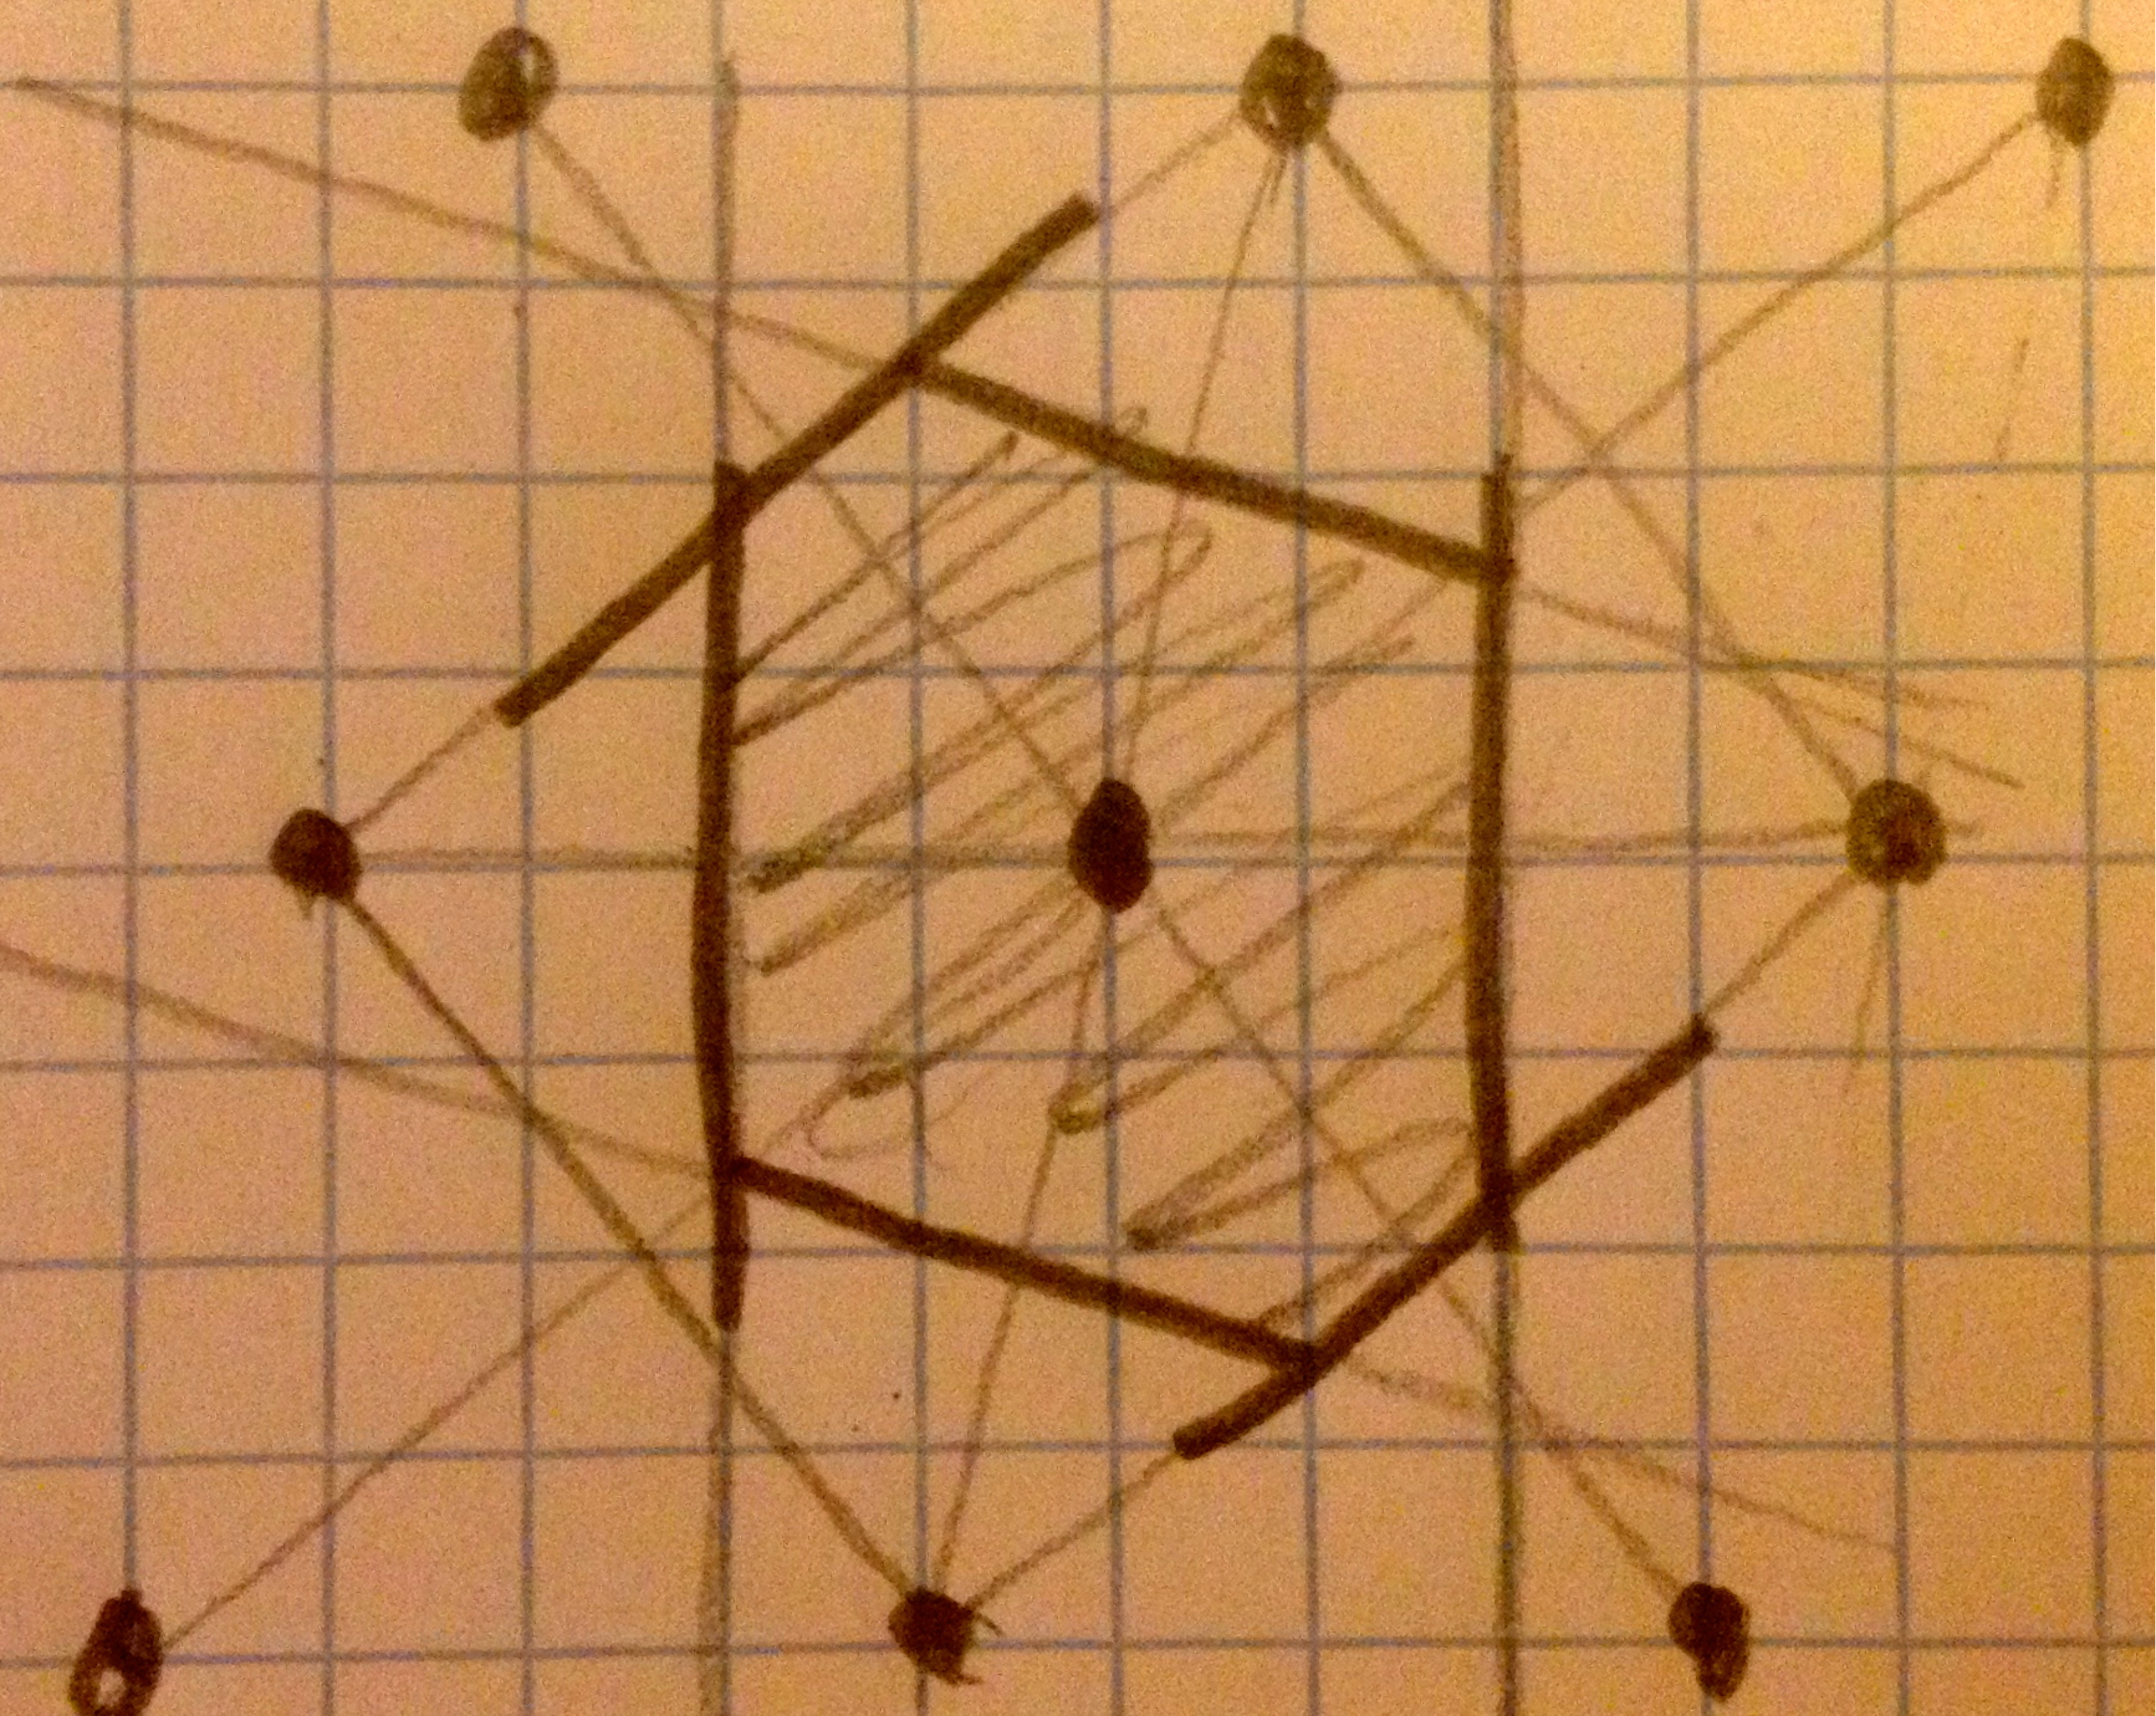
\includegraphics[width=0.45\linewidth]{./images/30_parallel}
			\caption{Brillouin Zonen eines Parallelogrammgitters}
		\end{figure}
		
	\end{karte}


%%%%%%%%%%%%%%%%%%%%%%%%%%%%%%%%%%%%%%%%%%%%%%%%%%%%%%%%%%%%%%%%%%%%%%%%%%
	\begin{karte}{
		Skizziere die Brillouinsche Zone eines 2D hexagonalen Gitters.
		}
		
		beschreiben symmetrische Polyeder im reziproken Gitter.
		
		\begin{figure}[htbp]
			\centering
			\includegraphics[width=0.45\linewidth]{./images/31_hex}
			\caption{Brillouin Zonen eines 2D hexagonalen Gitters}
		\end{figure}
		
	\end{karte}


%%%%%%%%%%%%%%%%%%%%%%%%%%%%%%%%%%%%%%%%%%%%%%%%%%%%%%%%%%%%%%%%%%%%%%%%%%
	\begin{karte}{
		Strukturfaktor / Atomfaktor.
		}
		
		Der Atomfaktor $f_\alpha$ beschreibt die Stärke der Streuung an einem Atom. \\ \\
		
		Der Strukturfaktor beschreibt die Interferenz zwischen Streuwellen von verschiedenen Atomen der Elementarzelle.
		
	\end{karte}


%%%%%%%%%%%%%%%%%%%%%%%%%%%%%%%%%%%%%%%%%%%%%%%%%%%%%%%%%%%%%%%%%%%%%%%%%%
	\begin{karte}{
		Unterschiede im Strukturfaktor im einfachen kubischen und im bcc-Gitter?
		}
		
		\begin{itemize}
			\item einfach kubisch
				$$   F_{hkl} = 
				\begin{cases}
					f_1 + f_2 & \mbox{für } h+k+l \mbox{ gerade}\\
					f_1 - f_2 &  \mbox{für } h+k+l \mbox{ ungerade}
				\end{cases}
				$$
			\item body-centered cubic (bcc)
				$$   F_{hkl} = 
				\begin{cases}
					2f	&	\mbox{für } h+k+l \mbox{ gerade}\\
					0	&	\mbox{für } h+k+l \mbox{ ungerade}
				\end{cases}
				$$
				es kommt zur (totalen) Auslöschung bestimmter Reflexe im bcc Gitter!
		\end{itemize}
		
	\end{karte}


%%%%%%%%%%%%%%%%%%%%%%%%%%%%%%%%%%%%%%%%%%%%%%%%%%%%%%%%%%%%%%%%%%%%%%%%%%
	\begin{karte}{
		Was führt zum Auslöschen bestimmter Reflexe in eimen bcc?
		}
		
		Die Auslöschungsregel des bcc Gitters ist geometrisch leicht zu verstehen. \\
		
		Die roten Atome kommen dazu - wir haben einfach doppelt so viele, aus Sicht des Kristalls identische Ebenen, wie im simplen kubischen Gitter. \\
		
		Die an den roten Atomen der zusätzlichen Ebenen reflektierte Welle ist genau in Antiphase zur Welle eins drüber und wird also immer für Auslöschung sorgen.
		
		\begin{figure}[htbp]
			\centering
			\includegraphics[width=0.45\linewidth]{./images/33_bcc}
			\caption{Auslöschung bei bcc Gitter}
		\end{figure}
		
	\end{karte}


%%%%%%%%%%%%%%%%%%%%%%%%%%%%%%%%%%%%%%%%%%%%%%%%%%%%%%%%%%%%%%%%%%%%%%%%%%
	\begin{karte}{
		Dispersionsrelation einer zweiatomigen linearen Kette. (Phononendispersion)
		}
		
		AAAAAARGH!!! \\
		
	\end{karte}


%%%%%%%%%%%%%%%%%%%%%%%%%%%%%%%%%%%%%%%%%%%%%%%%%%%%%%%%%%%%%%%%%%%%%%%%%%
	\begin{karte}{
		Unterschied akustische und optische Phononen.
		}
		
		Phononen: Quasiteilchen, delokalisiert, existieren im ganzen Gitter
		
		\begin{itemize}
			\item akustische Phononen
				\begin{itemize}
					\item entsprechen Schallwellen, die sich im Kristallgitter fortplanzen
					\item alle Atome einer Basis schwingen in Phase
				\end{itemize}
			\item optische Phononen 
				\begin{itemize}
					\item gegenphasige Bewegung
					\item Schwingung im Infrarotbereich
					\item Festkörper ncht zwingend optisch aktiv
					\item Beispiel: Ionengitter ($\ce{NaCl}$ Kristall)
				\end{itemize}
		\end{itemize}
		
		\begin{figure}[htbp]
			\centering
			\includegraphics[width=0.3\linewidth]{./images/36_phononen}
			\caption{Unterschied akustische und optische Phononen}
		\end{figure}
		
	\end{karte}


%%%%%%%%%%%%%%%%%%%%%%%%%%%%%%%%%%%%%%%%%%%%%%%%%%%%%%%%%%%%%%%%%%%%%%%%%%
	\begin{karte}{
		Wodurch unterscheiden sich die Dispersionsrelationen für Phononen im primitiv 
		kubischen Gitter und der $\ce{CsCl}$ Struktur (bcc kubisch raumzentriert.)?
		}
		
		\begin{itemize}
			\item jeder Kristall hat 3 akkustische Zweige
			\item für jedes zusätzliche Atom in Einheitszelle kommen 3 optische Zweige dazu
			\item primitiv kubisch (sc)
				\begin{itemize}
					\item 1 Atom/EZ $\Rightarrow$ 3 akkustische Zweige
				\end{itemize}
			\item kubisch raumzentriert (bcc)
				\begin{itemize}
					\item 2 Atom/EZ $\Rightarrow$ 3 akkustische Zweige + 3 optische Zweige
				\end{itemize}
		\end{itemize}
		
	\end{karte}


%%%%%%%%%%%%%%%%%%%%%%%%%%%%%%%%%%%%%%%%%%%%%%%%%%%%%%%%%%%%%%%%%%%%%%%%%%
	\begin{karte}{
		Zustandsdichte vom freien Elektronengases?
		}
		
		Die Zustandsdichte $D(E)$ gibt die Zahl der möglichen Energiezustände pro Energieeinheit an. \\

		\begin{itemize}
			\item 1D:  $  D(E) = \frac{L}{2\pi} \left( \frac{2m}{\hbar^2} \right)^{3/2} \frac{1}{\sqrt{E}}   $
			\item 3D:  $  D(E) = \frac{V}{2\pi^2} \left( \frac{2m}{\hbar^2} \right)^{3/2} \sqrt{E}   $
		\end{itemize}
		
		
	\end{karte}


%%%%%%%%%%%%%%%%%%%%%%%%%%%%%%%%%%%%%%%%%%%%%%%%%%%%%%%%%%%%%%%%%%%%%%%%%%
	\begin{karte}{
		Fermi-Verteilung für T = 0K und bei endlichen Temperaturen.
		}
		
		Die Fermi-Verteilung gibt an, mit welcher Wahrscheinlichkeit ein Fermion (z.B. ein Elektron) bei einer gegebenen Temperatur $T$ einen Zustand mit der Energie $E$ besetzen kann.
		
		\begin{itemize}
			\item $T=0K$ \\
				Das Pauli-Prinzip besagt, dass Fermionen nicht in allen Quantenzahlen übereinstimmen dürfen. Dies hat zur Folge, dass auch am absoluten Temperaturnullpunkt Fermionen in angeregten Energiezuständen sitzen müssen. \\
				Die Fermi-Verteilung hat bei $T=0K$ also eine scharfe Kante bei einer Energie, deren Höhe von der Anzahl der Fermionen in dem betrachteten System abhängt und als Fermi-Kante oder Fermi-Energie $E_f$ bezeichnet wird. Ganz wichtig ist hierbei, dass die Fermi-Verteilung nur eine Wahrscheinlichkeit angibt, mit der ein Zustand besetzt wird. Ob der Zustand auch besetzt wird, hängt davon ab, ob ein entsprechender Zustand existiert \\
				$$f(E,T=0K)= \begin{cases}
					1 & \mbox{Alle Zustände unter der Fermi-Energie sind mit Fermionen besetzt} \\
					0 & \mbox{Zustände oberhalb der Fermi-Energie sind nicht von Fermionen besetzt}
				\end{cases}$$
			\item $T>0K$ \\
				$$f(E,T) = \frac{ 1 }{  \exp \left( \frac{ E- \mu }{k_B T} \right) + 1   } $$
		\end{itemize}
		
	\end{karte}


%%%%%%%%%%%%%%%%%%%%%%%%%%%%%%%%%%%%%%%%%%%%%%%%%%%%%%%%%%%%%%%%%%%%%%%%%%
	\begin{karte}{
		Entstehung elektronischer Bänder im Festkörper.
		}
		
		Im Festkoörper wechselwirken eine Vielzahl von Elektronen miteinander, wodurch immer mehr Energieniveaus entstehen, die als Energiebänder zusammengefasst werden.
		
	\end{karte}


%%%%%%%%%%%%%%%%%%%%%%%%%%%%%%%%%%%%%%%%%%%%%%%%%%%%%%%%%%%%%%%%%%%%%%%%%%
	\begin{karte}{
		Bildung elektronischer Bänder mit der Methode des ”stark gebundenen“ Elektrons. 
		(”tight binding“ Näherung)
		}
		
		ääähm…
		
	\end{karte}


%%%%%%%%%%%%%%%%%%%%%%%%%%%%%%%%%%%%%%%%%%%%%%%%%%%%%%%%%%%%%%%%%%%%%%%%%%
	\begin{karte}{
		Wovon hängt die Breite von elektronischen Bändern ab?
		}
		
		Die Breite hängt vom Überlapp der benachbarten Wellenfunktionen ab. Diese wiederum hängt von der Lokalisierung ab:
		\begin{itemize}
			\item lokalisiert $\Rightarrow$ schmale Bänder
			\item delokalisiert $\Rightarrow$ breite Bänder
		\end{itemize}
		
	\end{karte}


%%%%%%%%%%%%%%%%%%%%%%%%%%%%%%%%%%%%%%%%%%%%%%%%%%%%%%%%%%%%%%%%%%%%%%%%%%
	\begin{karte}{
		Wann ist ein Festkörper Leiter bzw. Nichtleiter?
		}
		
		Wenn die Fermi-Energie innerhalb eines Energiebandes liegt sind nicht alle Energiezustände in diesem Band besetzt.
		
		Damit könne Elektronen beim Anlegen einer Spannung Energie aufnehmen und sich in Richtung des elktrischen Feldes bewegen.
		
		Diese Festkörper sind elektrische Leiter.
		
	\end{karte}

%%%%%%%%%%%%%%%%%%%%%%%%%%%%%%%%%%%%%%%%%%%%%%%%%%%%%%%%%%%%%%%%%%%%%%%%%%


\end{document}

